\documentclass[conference]{IEEEtran}
\IEEEoverridecommandlockouts

\usepackage[utf8]{inputenc}
\usepackage[T5]{fontenc}
\usepackage[vietnamese]{babel}
\usepackage{cite}
\usepackage{amsmath,amssymb,amsfonts}
\usepackage{graphicx}
\usepackage{textcomp}
\usepackage{xcolor}
\usepackage{booktabs}
\usepackage{multirow}
\usepackage{url}
\usepackage{hyperref}
\usepackage{float}
\usepackage{listings}

% Cấu hình code listing
\lstset{
    language=Python,
    basicstyle=\ttfamily\small,
    keywordstyle=\color{blue},
    stringstyle=\color{red},
    commentstyle=\color{green!60!black},
    backgroundcolor=\color{gray!10},
    showspaces=false,
    showstringspaces=false,
    frame=single,
    tabsize=2,
    breaklines=true,
    breakatwhitespace=false,
}

\begin{document}

% ======================== TRANG BÌA ========================
\begin{titlepage}
\begin{center}

\vspace*{3cm}

{\Large\bfseries NHẬN DẠNG CỬ CHỈ TAY PHỤC VỤ ĐIỀU KHIỂN\\[0.3cm]
THIẾT BỊ HỖ TRỢ CHĂM SÓC BỆNH NHÂN\\[0.3cm]
TRONG PHÒNG BỆNH THÔNG MINH}

\vspace{1.5cm}

{\large Nhóm 11}

\vspace{0.5cm}

{\large Đại Nam University\\
Hà Nội, Việt Nam}

\vspace{1cm}

{\large MỤC LỤC}

\end{center}
\end{titlepage}

% (Đã bỏ mục lục theo yêu cầu)

% ======================== NỘI DUNG CHÍNH ========================
\title{Nhận dạng cử chỉ tay phục vụ điều khiển\\thiết bị hỗ trợ chăm sóc bệnh nhân\\trong phòng bệnh thông minh}

\author{
\IEEEauthorblockN{Nhóm 11}
\IEEEauthorblockA{Đại Nam University\\
Hà Nội, Việt Nam}
}

\maketitle

\begin{abstract}
Trong môi trường y tế hiện đại, việc hỗ trợ bệnh nhân tương tác với các thiết bị trong phòng bệnh mà không cần tiếp xúc vật lý là nhu cầu cấp thiết, đặc biệt tại các phòng hồi sức tích cực. Bài báo đề xuất hệ thống nhận dạng cử chỉ tay thời gian thực sử dụng mô hình YOLOv8 Nano để điều khiển thiết bị hỗ trợ chăm sóc bệnh nhân trong phòng bệnh thông minh. Hệ thống nhận dạng 3 cử chỉ tay chính: \textbf{Nắm tay} (bật/tắt đèn), \textbf{Chỉ ngón trỏ} (điều chỉnh giường bệnh) và \textbf{Xòe tay} (báo động khẩn cấp SOS). Bộ dữ liệu tự thu thập gồm 2.561 ảnh được gán nhãn bounding box trên Roboflow và huấn luyện trên Google Colab với GPU Tesla T4. Kết quả thực nghiệm cho thấy mô hình đạt Precision \textbf{97,5\%}, Recall \textbf{97,4\%} và mAP@0.5 đạt \textbf{98,8\%} trên tập validation. Hệ thống tích hợp bộ lọc Dwell-time 5 giây chống kích hoạt nhầm và phản hồi bằng giọng nói, đảm bảo hoạt động ổn định ở 30 FPS trên thiết bị cấu hình trung bình.
\end{abstract}

\begin{IEEEkeywords}
nhận dạng cử chỉ tay, YOLOv8, phòng bệnh thông minh, điều khiển không tiếp xúc, học sâu, IoT y tế
\end{IEEEkeywords}

\section{Đặt vấn đề}

Trong môi trường y tế hiện đại, đặc biệt tại các phòng bệnh hồi sức tích cực hoặc phòng chăm sóc bệnh nhân đặc biệt, khả năng tương tác của bệnh nhân với môi trường xung quanh gặp nhiều hạn chế. Việc sử dụng các nút bấm vật lý truyền thống gặp các trở ngại: khó tiếp cận đối với bệnh nhân bị liệt một phần, nguy cơ lây nhiễm chéo vi khuẩn/virus qua các bề mặt tiếp xúc, hoặc không tiện dụng trong các tình huống khẩn cấp.

Giao tiếp bằng cử chỉ tay là phương thức tự nhiên và trực quan cho con người. Nhiều nghiên cứu đã chứng minh tính khả thi của việc nhận dạng cử chỉ tay bằng thị giác máy tính trong các ứng dụng tương tác người--máy \cite{ref1}. Tuy nhiên, hầu hết các hệ thống hiện có tập trung vào ngữ cảnh giải trí hoặc công nghiệp mà chưa đáp ứng đặc thù của môi trường y tế --- nơi đòi hỏi độ tin cậy cao, phản hồi thời gian thực và cơ chế an toàn chống kích hoạt nhầm.

Để giải quyết bài toán trên, dự án này đề xuất xây dựng hệ thống \textbf{Smart Hospital Assistant} --- hỗ trợ bệnh nhân điều khiển các thiết bị cơ bản trong phòng bệnh thông qua cử chỉ tay không tiếp xúc. Hệ thống sử dụng camera thu thập luồng hình ảnh trực tiếp, nhận dạng cử chỉ bằng mô hình học sâu YOLOv8 \cite{ref7} và thực thi lệnh tương ứng.

Bài báo có ba đóng góp chính:

\begin{enumerate}
    \item \textbf{Xây dựng bộ dữ liệu cử chỉ tay chuyên biệt cho y tế:} Thu thập và gán nhãn 2.561 ảnh bao gồm 3 lớp cử chỉ hành động và ảnh nền (negative samples), phản ánh đa dạng điều kiện thực tế phòng bệnh.
    \item \textbf{Thiết kế kiến trúc nhận dạng thời gian thực:} Sử dụng YOLOv8 Nano kết hợp bộ lọc chống nhiễu Anti-flicker và cơ chế Dwell-time 5 giây, đảm bảo an toàn tuyệt đối trong ngữ cảnh y tế.
    \item \textbf{Triển khai ứng dụng hoàn chỉnh:} Xây dựng giao diện Dashboard y tế tích hợp phản hồi giọng nói (Text-to-Speech) và điều khiển giả lập thiết bị phòng bệnh.
\end{enumerate}

\section{Các nghiên cứu liên quan}

Nhận dạng cử chỉ tay là một lĩnh vực nghiên cứu quan trọng trong thị giác máy tính và tương tác người--máy. Các phương pháp tiếp cận có thể phân thành hai nhóm chính: dựa trên đặc trưng thủ công và dựa trên học sâu.

\textbf{Phương pháp dựa trên đặc trưng thủ công:} Các nghiên cứu ban đầu sử dụng MediaPipe Hands để trích xuất 21 điểm mốc (landmarks) trên bàn tay, sau đó áp dụng các bộ phân loại truyền thống như Random Forest, K-Nearest Neighbors hoặc SVM \cite{ref1}. Phương pháp này có ưu điểm nhẹ nhàng nhưng phụ thuộc nhiều vào chất lượng phát hiện landmark và không có khả năng định vị vùng tay trong ảnh.

\textbf{Phương pháp dựa trên học sâu:} Các mô hình CNN như ResNet \cite{ref9}, EfficientNet đã chứng minh hiệu quả cao trong phân loại cử chỉ. Vision Transformer (ViT) \cite{ref5} và ConvNeXt \cite{ref3} đạt hiệu năng vượt trội trên các bộ dữ liệu lớn. Tuy nhiên, các mô hình phân loại thuần túy không cung cấp thông tin vị trí (bounding box) của bàn tay --- yếu tố cần thiết cho ứng dụng thời gian thực.

\textbf{Phát hiện đối tượng (Object Detection):} Họ YOLO \cite{ref2} giải quyết đồng thời bài toán định vị và phân loại trong một lần quét ảnh duy nhất, phù hợp cho ứng dụng thời gian thực. YOLOv8 \cite{ref7} là phiên bản mới nhất với nhiều cải tiến về kiến trúc backbone CSPDarknet, neck PANet và detection head anchor-free. Phiên bản Nano (YOLOv8n) với chỉ 3 triệu tham số cho phép triển khai trên các thiết bị biên (edge devices) với tốc độ suy luận cao.

Trong bối cảnh phòng bệnh thông minh, một số nghiên cứu đã ứng dụng nhận dạng cử chỉ để điều khiển thiết bị \cite{ref1}, \cite{ref4}. Tuy nhiên, hầu hết chưa giải quyết triệt để vấn đề kích hoạt nhầm --- đặc biệt nguy hiểm trong môi trường y tế. Nghiên cứu này đề xuất cơ chế Dwell-time kết hợp Anti-flicker buffer để đảm bảo an toàn tuyệt đối.

\begin{figure}[h]
\centering
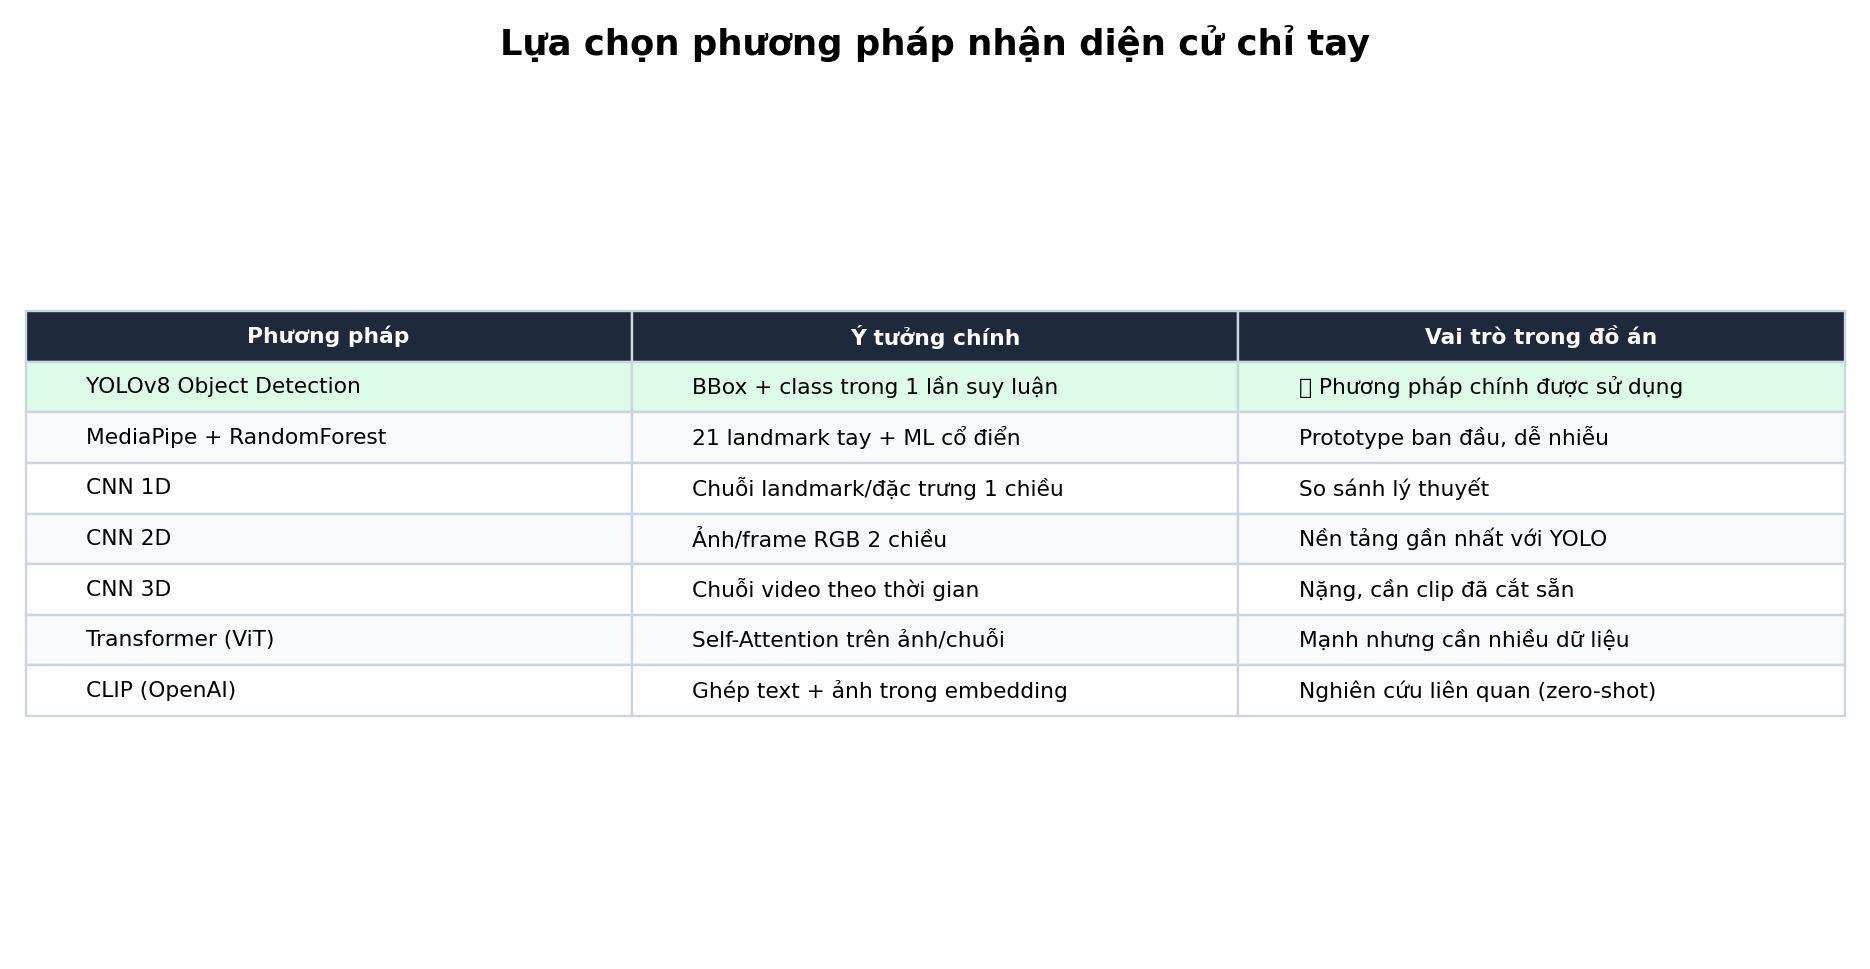
\includegraphics[width=\columnwidth]{figures/method_selection.png}
\caption{So sánh các phương pháp nhận dạng cử chỉ tay. YOLO object detection được lựa chọn vì đáp ứng đồng thời yêu cầu định vị + phân loại thời gian thực.}
\label{fig:method_selection}
\end{figure}

\begin{figure}[h]
\centering
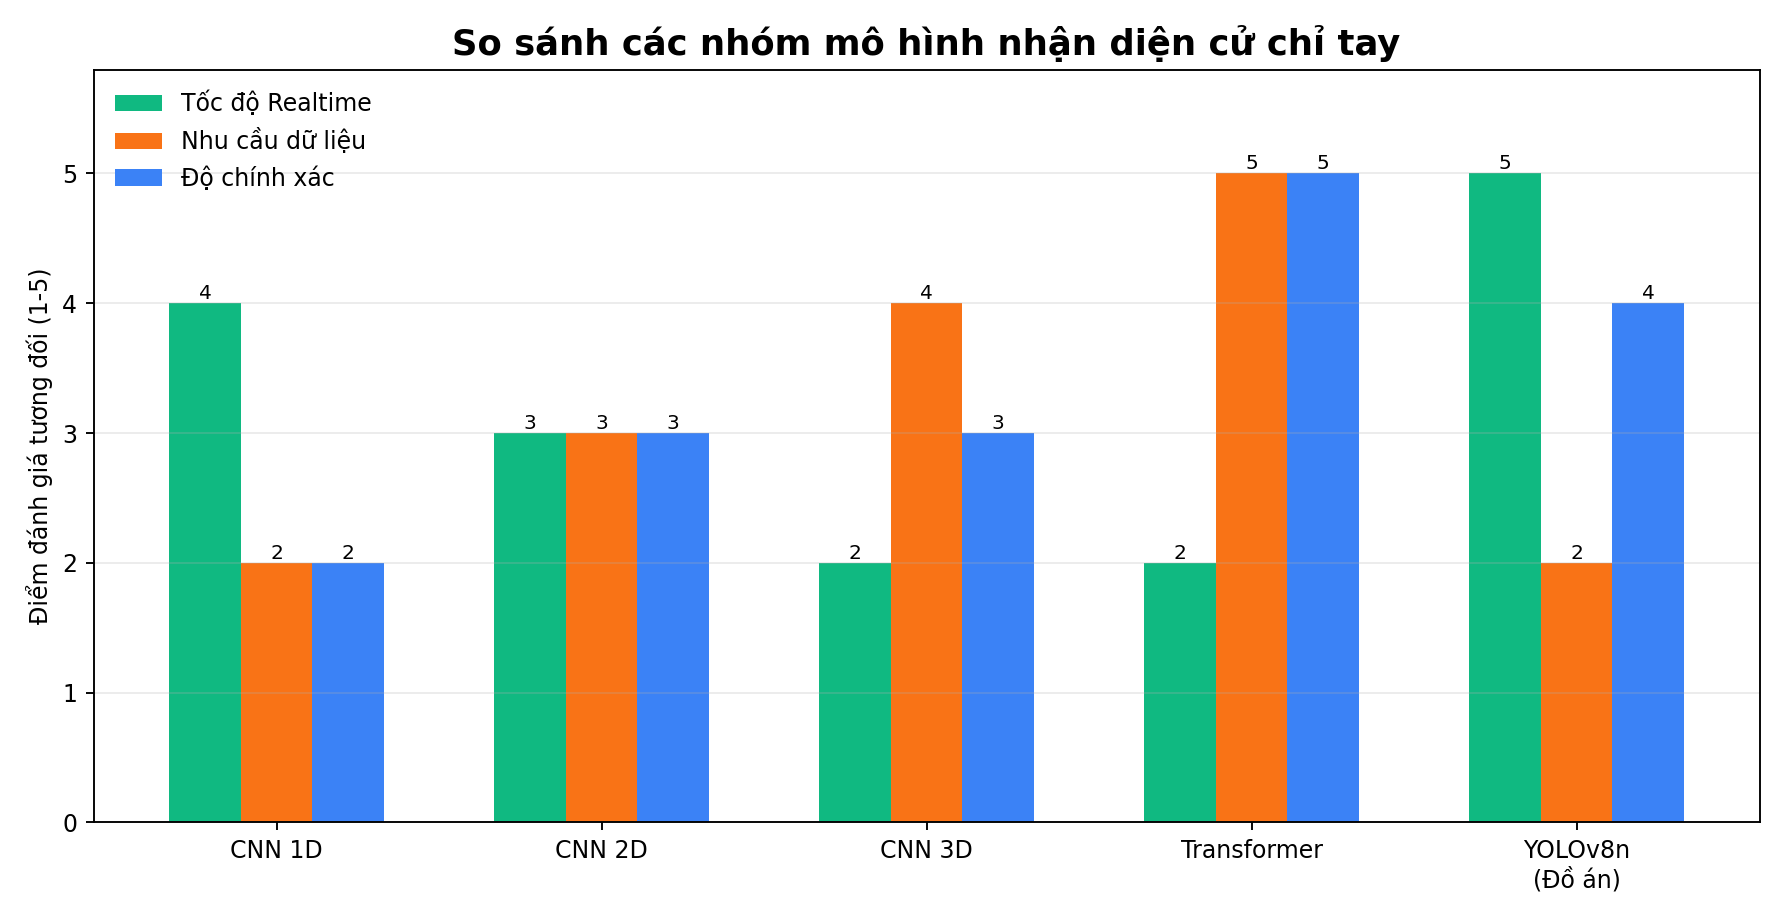
\includegraphics[width=\columnwidth]{figures/model_family_comparison.png}
\caption{So sánh các họ mô hình: CNN 1D, CNN 2D, CNN 3D, Transformer và YOLO. YOLOv8 Nano cân bằng tốt nhất giữa độ chính xác, tốc độ và kích thước mô hình.}
\label{fig:model_comparison}
\end{figure}

\section{Xây dựng bộ dữ liệu và tiền xử lý}

\subsection{Thu thập dữ liệu}

Dữ liệu được thu thập bằng cách quay video trực tiếp các hành vi cử chỉ tay dưới nhiều góc độ, khoảng cách và điều kiện ánh sáng khác nhau để tăng tính tổng quát hóa. Mỗi cử chỉ được quay thành file video riêng biệt: \texttt{nam\_tay.mp4}, \texttt{chi\_ngon.mp4}, \texttt{xoe\_tay.mp4} và \texttt{binh\_thuong.mp4}. Video sau đó được trích xuất thành ảnh tĩnh bằng script tự động:

\begin{lstlisting}[caption={Trích xuất frame từ video}]
python training/01_extract_frames.py \
    --every-n 6 --max-per-video 800
\end{lstlisting}

\subsection{Gán nhãn dữ liệu trên Roboflow}

Toàn bộ ảnh được tải lên nền tảng Roboflow để vẽ hộp bao (bounding box) quanh bàn tay. Quy tắc gán nhãn:
\begin{itemize}
    \item Hộp bao ôm sát phần bàn tay và cổ tay.
    \item Loại bỏ ảnh mờ, mất tay hoặc ánh sáng quá tệ.
    \item Thống nhất 1 tay chính trong toàn bộ dataset.
    \item Export định dạng YOLOv8 để huấn luyện.
\end{itemize}

\subsection{Các lớp cử chỉ (Classes)}

Hệ thống triển khai 3 lớp cử chỉ hành động chính và trạng thái nghỉ:

\begin{table}[h]
\centering
\caption{Định nghĩa các lớp cử chỉ và hành động tương ứng}
\label{tab:classes}
\begin{tabular}{c|l|l|l}
\hline
\textbf{ID} & \textbf{Tên class} & \textbf{Cử chỉ} & \textbf{Hành động} \\
\hline
0 & Binh\_Thuong & Tay nghỉ & Không kích hoạt \\
1 & Nam\_Tay & Nắm tay & Bật/tắt đèn \\
2 & Chi\_Ngon\_Tro & Chỉ ngón trỏ & Chỉnh giường \\
3 & Xoe\_Tay & Xòe tay & SOS khẩn cấp \\
\hline
\end{tabular}
\end{table}

\subsection{Chiến lược xử lý trạng thái nghỉ}

Để loại bỏ cảnh báo giả khi bệnh nhân không thực hiện cử chỉ nào, các ảnh thuộc lớp ``Bình thường'' không được gán nhãn mà đưa vào mô hình dưới dạng \textbf{Background images (Negative samples)} --- file nhãn \texttt{.txt} tương ứng hoàn toàn trống. YOLOv8 sẽ học cách phớt lờ bàn tay thả lỏng, giảm thiểu tỉ lệ False Positive.

\subsection{Thống kê phân bố tập dữ liệu}

\begin{table}[h]
\centering
\caption{Phân bổ dữ liệu Train/Val}
\label{tab:dataset}
\begin{tabular}{l|c|c|c}
\hline
\textbf{Lớp cử chỉ} & \textbf{Train (80\%)} & \textbf{Val (20\%)} & \textbf{Tổng} \\
\hline
Nam\_Tay & 483 & 121 & 604 \\
Chi\_Ngon\_Tro & 448 & 112 & 560 \\
Xoe\_Tay & 625 & 156 & 781 \\
Ảnh nền (Background) & 493 & 123 & 616 \\
\hline
\textbf{Tổng cộng} & \textbf{2.049} & \textbf{512} & \textbf{2.561} \\
\hline
\end{tabular}
\end{table}

\begin{figure}[h]
\centering
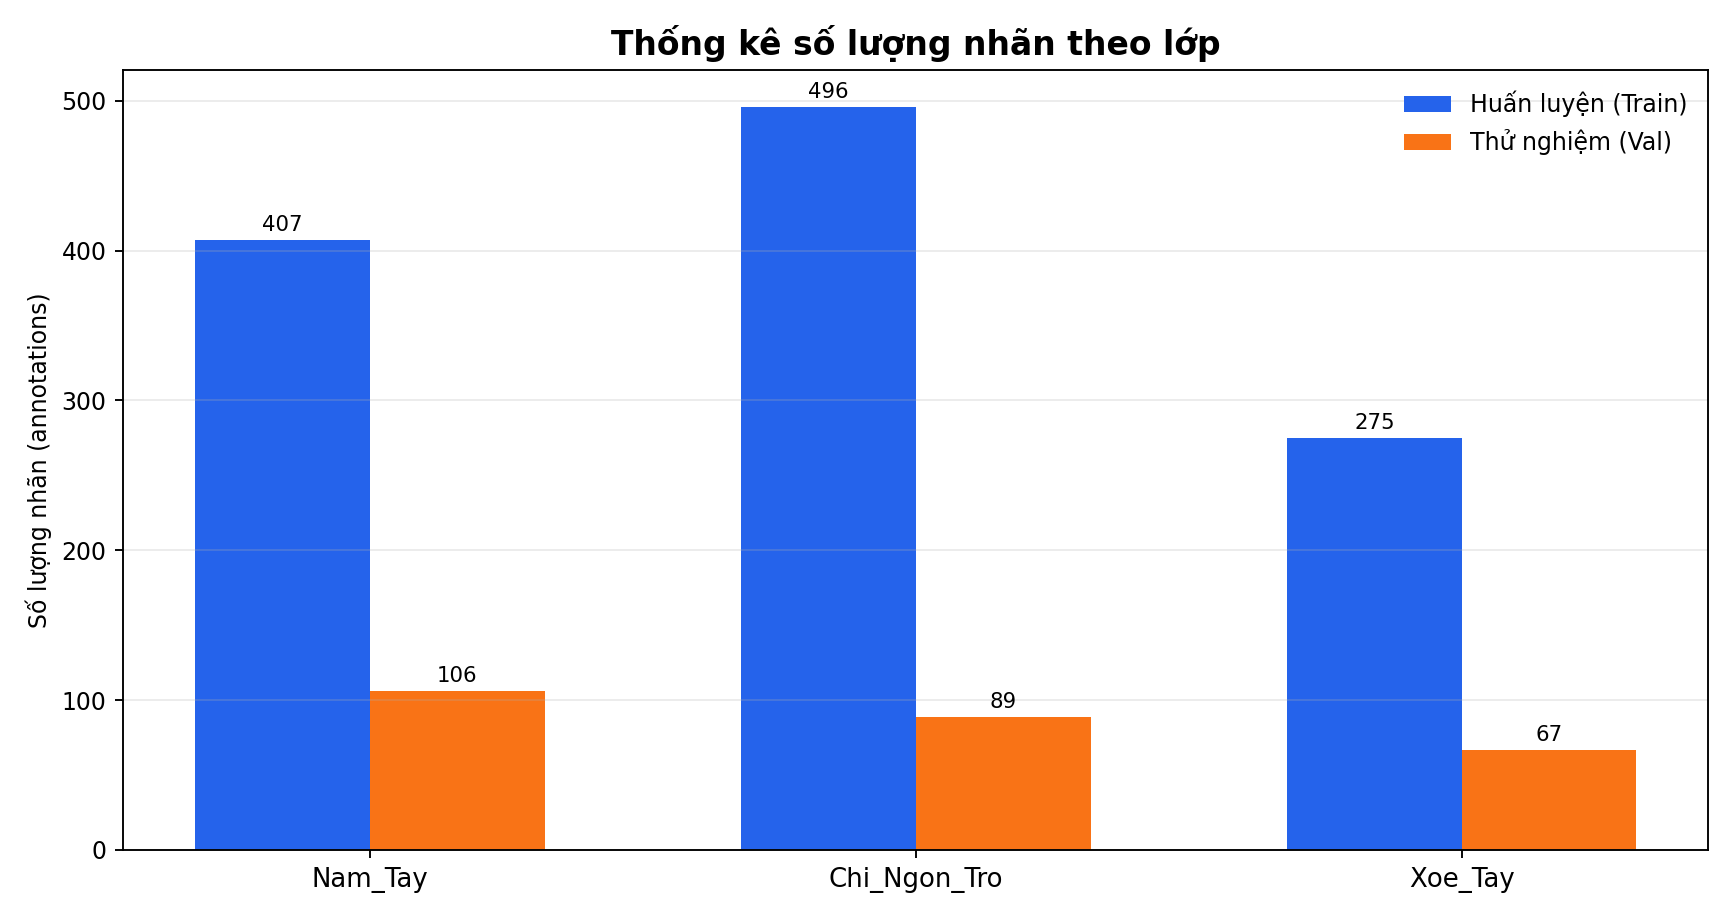
\includegraphics[width=\columnwidth]{figures/class_distribution.png}
\caption{Biểu đồ phân bố số lượng ảnh theo lớp cử chỉ. Bộ dữ liệu được thiết kế với sự cân bằng giữa các lớp nhằm hạn chế hiện tượng thiên vị lớp.}
\label{fig:distribution}
\end{figure}

\begin{figure}[h]
\centering
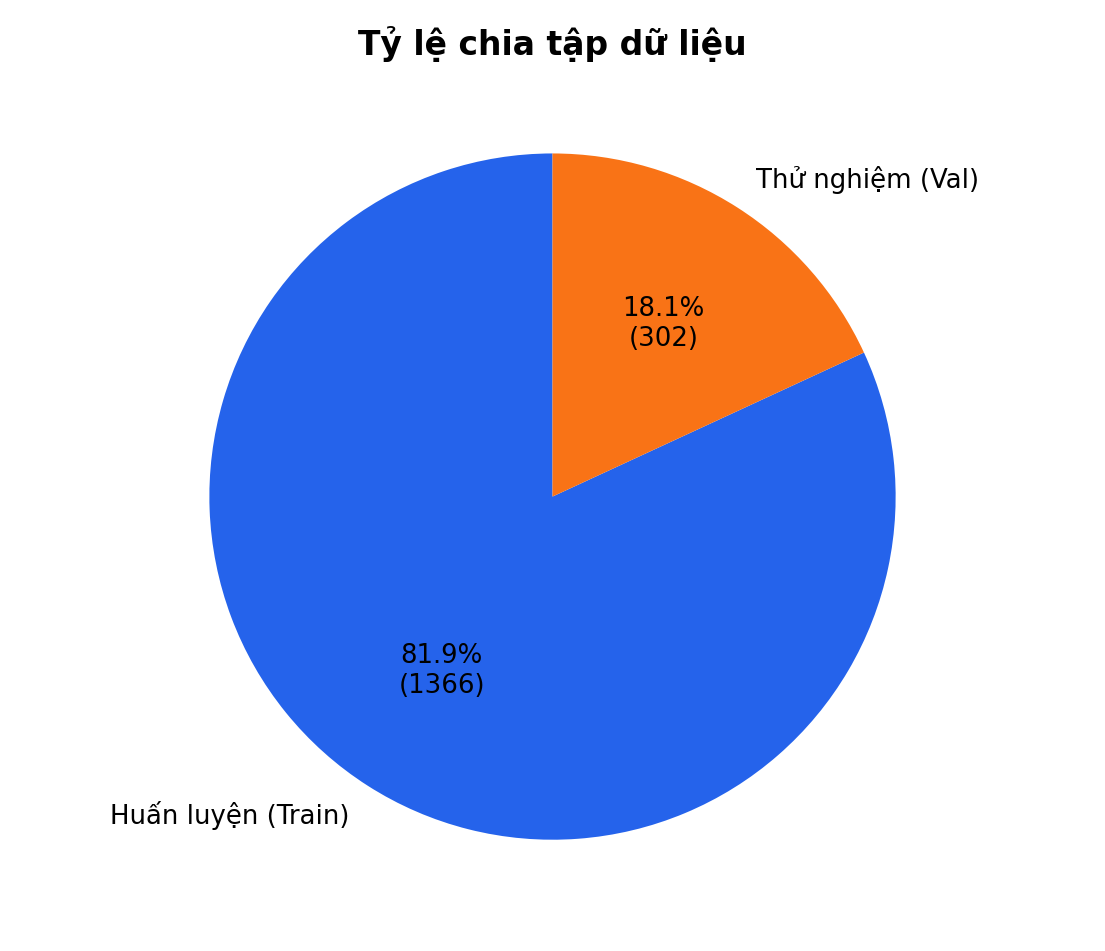
\includegraphics[width=\columnwidth]{figures/split_distribution.png}
\caption{Phân bố dữ liệu train/val theo lớp cử chỉ, đảm bảo stratified split cân bằng giữa tập huấn luyện và tập kiểm tra.}
\label{fig:split}
\end{figure}

\section{Kiến trúc hệ thống và luồng xử lý}

\subsection{Tổng quan kiến trúc}

Hệ thống được thiết kế theo mô hình luồng dữ liệu thời gian thực gồm 4 giai đoạn: (1) Thu nhận hình ảnh từ camera, (2) Nhận dạng cử chỉ qua YOLOv8, (3) Lọc chống nhiễu Dwell-time, (4) Điều khiển và phản hồi.

\begin{figure}[h]
\centering
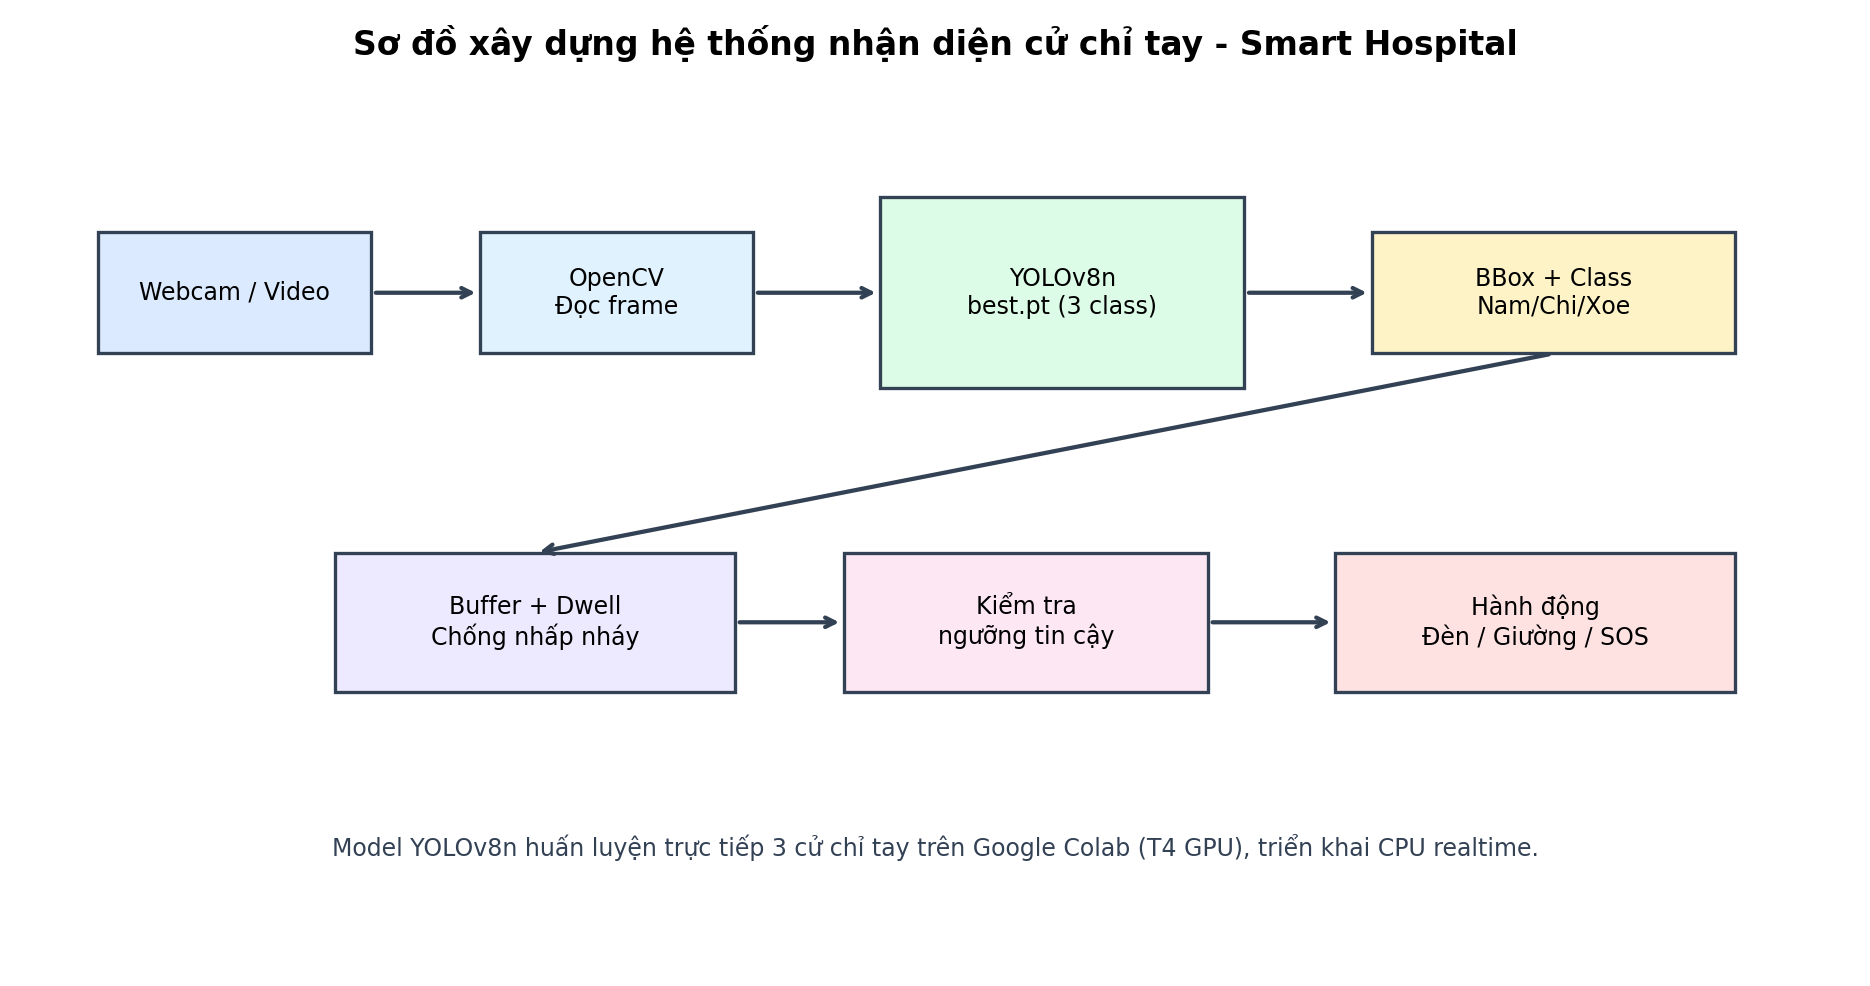
\includegraphics[width=\columnwidth]{figures/architecture_diagram.png}
\caption{Kiến trúc tổng thể hệ thống nhận dạng cử chỉ tay điều khiển phòng bệnh thông minh. Luồng xử lý từ Camera qua YOLOv8 đến Dashboard điều khiển.}
\label{fig:architecture}
\end{figure}

\subsection{Mô hình YOLOv8 Nano}

Chúng tôi lựa chọn kiến trúc \textbf{YOLOv8 Nano (yolov8n)} nhằm đảm bảo tốc độ phản hồi thời gian thực trên các thiết bị cấu hình trung bình. YOLOv8 \cite{ref7} là phiên bản mới nhất của họ YOLO với các cải tiến:

\begin{itemize}
    \item \textbf{Backbone:} CSPDarknet với Cross Stage Partial connections giúp giảm tham số mà vẫn giữ đặc trưng phong phú.
    \item \textbf{Neck:} PANet (Path Aggregation Network) kết hợp đặc trưng đa tỉ lệ.
    \item \textbf{Head:} Anchor-free detection head, loại bỏ anchor boxes thủ công.
    \item \textbf{Loss:} CIoU loss cho regression, BCE loss cho classification.
\end{itemize}

Đầu vào là ảnh RGB kích thước $640 \times 640$. Đầu ra gồm bounding box tọa độ $(x, y, w, h)$, nhãn class cử chỉ và confidence score.

\begin{figure}[h]
\centering
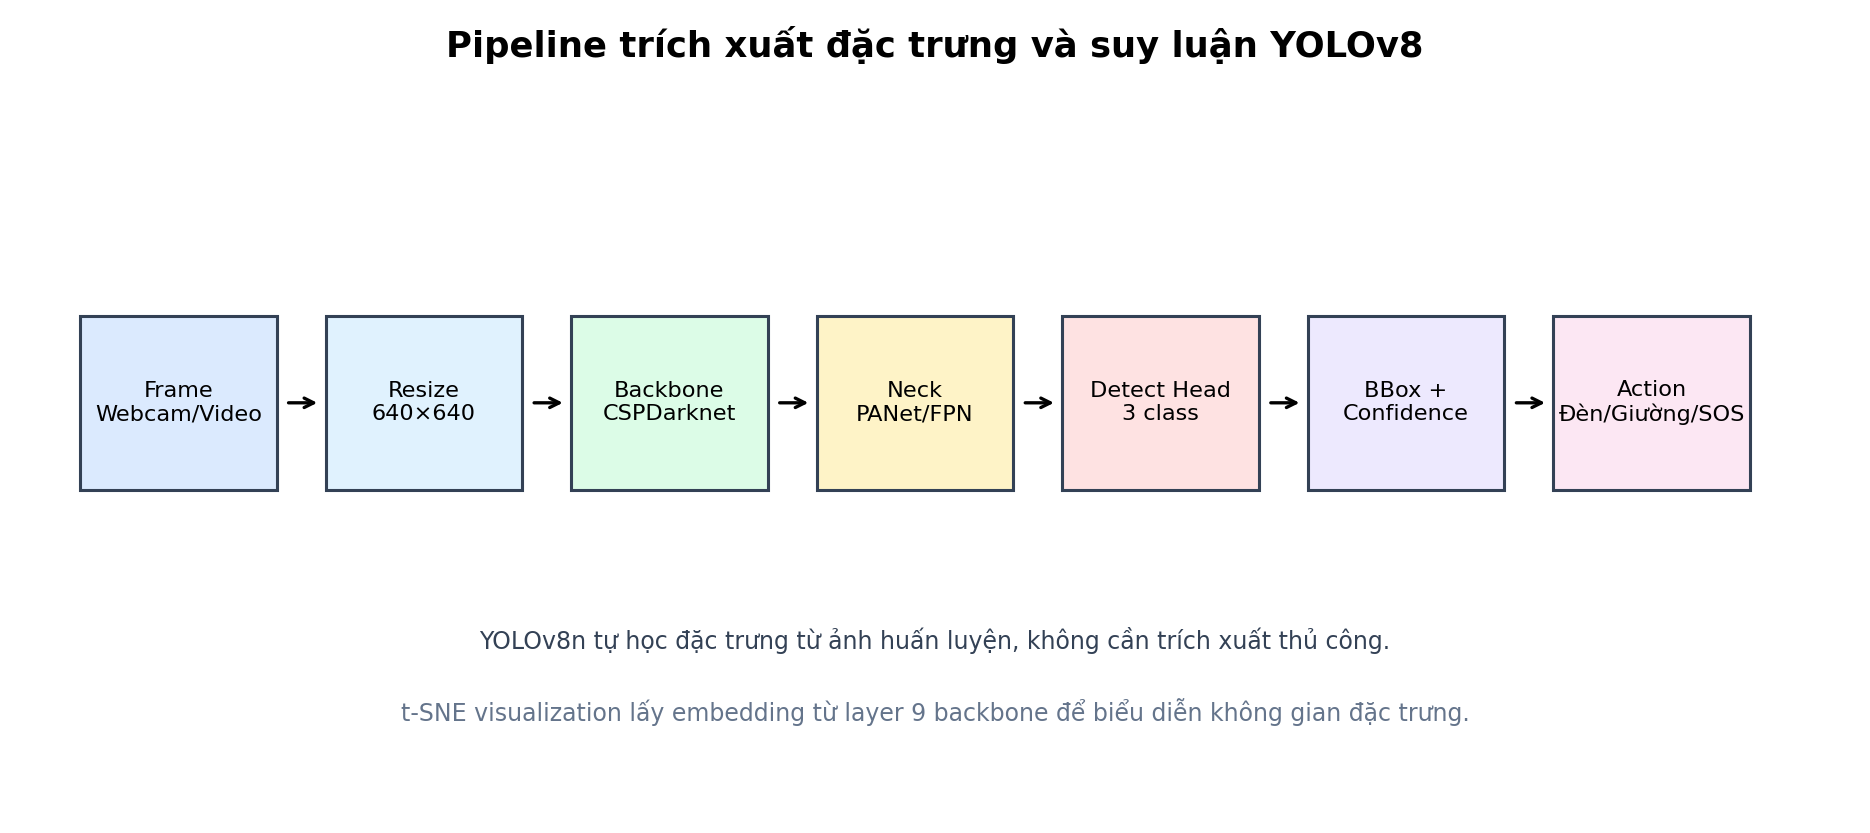
\includegraphics[width=\columnwidth]{figures/feature_extraction_pipeline.png}
\caption{Pipeline trích xuất đặc trưng: YOLOv8 backbone trích xuất feature maps, detection head trả về bounding box + class + confidence. Hệ thống map kết quả sang cử chỉ điều khiển.}
\label{fig:pipeline}
\end{figure}

\subsection{Bộ lọc chống nhiễu Anti-flicker và Dwell-time}

Trong môi trường y tế, kích hoạt nhầm có thể gây hậu quả nghiêm trọng. Chúng tôi thiết kế hai lớp bảo vệ:

\textbf{Lớp 1 --- Anti-flicker Buffer:} Sử dụng bộ đệm trượt 7 frame. Cử chỉ chỉ được xác nhận khi xuất hiện ổn định $\geq 4/7$ frame liên tiếp:
\begin{equation}
\text{stable}(t) = \begin{cases} g & \text{nếu } \text{count}(g, \text{buf}_7) \geq 4 \\ \text{stable}(t-1) & \text{ngược lại} \end{cases}
\end{equation}
trong đó $g$ là cử chỉ phổ biến nhất trong buffer 7 frame, $\text{buf}_7$ là cửa sổ trượt.

\textbf{Lớp 2 --- Dwell-time 5 giây:} Sau khi cử chỉ ổn định, bệnh nhân phải duy trì liên tục 5 giây trước khi hệ thống kích hoạt hành động:
\begin{equation}
\text{activate}(g) = \begin{cases} \text{true} & \text{nếu } t_{\text{hold}} \geq 5{,}0\text{s} \\ \text{false} & \text{ngược lại} \end{cases}
\end{equation}

Cơ chế này đảm bảo bệnh nhân thật sự có chủ đích, tránh kích hoạt do cử chỉ thoáng qua.

\subsection{Xử lý riêng cho SOS}

Đối với cử chỉ \textbf{Xòe tay} (SOS), khi đã kích hoạt, hệ thống phát cảnh báo lặp lại mỗi 3 giây cho đến khi bệnh nhân hạ tay:
\begin{equation}
\text{repeat\_SOS}(t) = \left[t - t_{\text{last\_sos}} > 3{,}0\text{s}\right] \land \left[\text{gesture} = \text{Xoe\_Tay}\right]
\end{equation}

\section{Huấn luyện mô hình}

\subsection{Thông số huấn luyện}

Mô hình được huấn luyện trên Google Colab với GPU Tesla T4. Các siêu tham số:

\begin{table}[h]
\centering
\caption{Siêu tham số huấn luyện}
\label{tab:hyperparams}
\begin{tabular}{l|c}
\hline
\textbf{Tham số} & \textbf{Giá trị} \\
\hline
Model gốc & yolov8n.pt \\
Số Epoch & 100 \\
Kích thước ảnh (imgsz) & 640 \\
Batch size & 16 \\
Thiết bị & GPU CUDA (T4) \\
Early Stopping (patience) & 20 \\
Optimizer & SGD + momentum \\
Learning rate & 0,01 \\
\hline
\end{tabular}
\end{table}

\subsection{Quá trình huấn luyện trên Colab}

Tiến trình huấn luyện được tự động hóa:

\begin{lstlisting}[caption={Lệnh huấn luyện YOLOv8}]
from ultralytics import YOLO

model = YOLO('yolov8n.pt')
results = model.train(
    data='data.yaml',
    epochs=100, imgsz=640,
    batch=16, device=0,
    patience=20,
    project='/content/runs',
    name='gesture_hospital_v1'
)
\end{lstlisting}

Pipeline hoàn chỉnh 6 giai đoạn:

\begin{table}[h]
\centering
\caption{Pipeline huấn luyện và triển khai}
\label{tab:pipeline}
\begin{tabular}{c|l|l}
\hline
\textbf{\#} & \textbf{Giai đoạn} & \textbf{Công cụ} \\
\hline
1 & Quay video cử chỉ & Webcam/Điện thoại \\
2 & Trích frame & \texttt{01\_extract\_frames.py} \\
3 & Gán nhãn bbox & Roboflow \\
4 & Đóng gói dataset & \texttt{02\_package\_dataset.py} \\
5 & Huấn luyện & Google Colab + GPU T4 \\
6 & Triển khai & Copy \texttt{best.pt} vào app \\
\hline
\end{tabular}
\end{table}

\section{Kết quả thực nghiệm và đánh giá}

\subsection{Độ chính xác mô hình}

Sau khi hoàn thành huấn luyện, mô hình được đánh giá trên tập validation độc lập 512 ảnh:

\begin{table}[h]
\centering
\caption{Chỉ số đánh giá mô hình trên tập Validation}
\label{tab:results}
\begin{tabular}{l|c|c|c|c}
\hline
\textbf{Lớp cử chỉ} & \textbf{P} & \textbf{R} & \textbf{mAP@0.5} & \textbf{mAP@0.5:0.95} \\
\hline
Toàn bộ (All) & 0,975 & 0,974 & 0,988 & 0,944 \\
Nam\_Tay & 0,968 & 0,943 & 0,977 & 0,916 \\
Chi\_Ngon\_Tro & 0,953 & 0,966 & 0,986 & 0,957 \\
Xoe\_Tay & 0,985 & 0,996 & 0,994 & 0,962 \\
\hline
\end{tabular}
\end{table}

Kết quả cho thấy mô hình đạt hiệu suất cao trên cả 3 lớp cử chỉ, với mAP@0.5 trung bình đạt \textbf{98,8\%}. Đặc biệt, cử chỉ \textbf{Xòe tay} (SOS) đạt Recall cao nhất (99,6\%) --- đảm bảo không bỏ sót tín hiệu cấp cứu.

\begin{figure}[h]
\centering
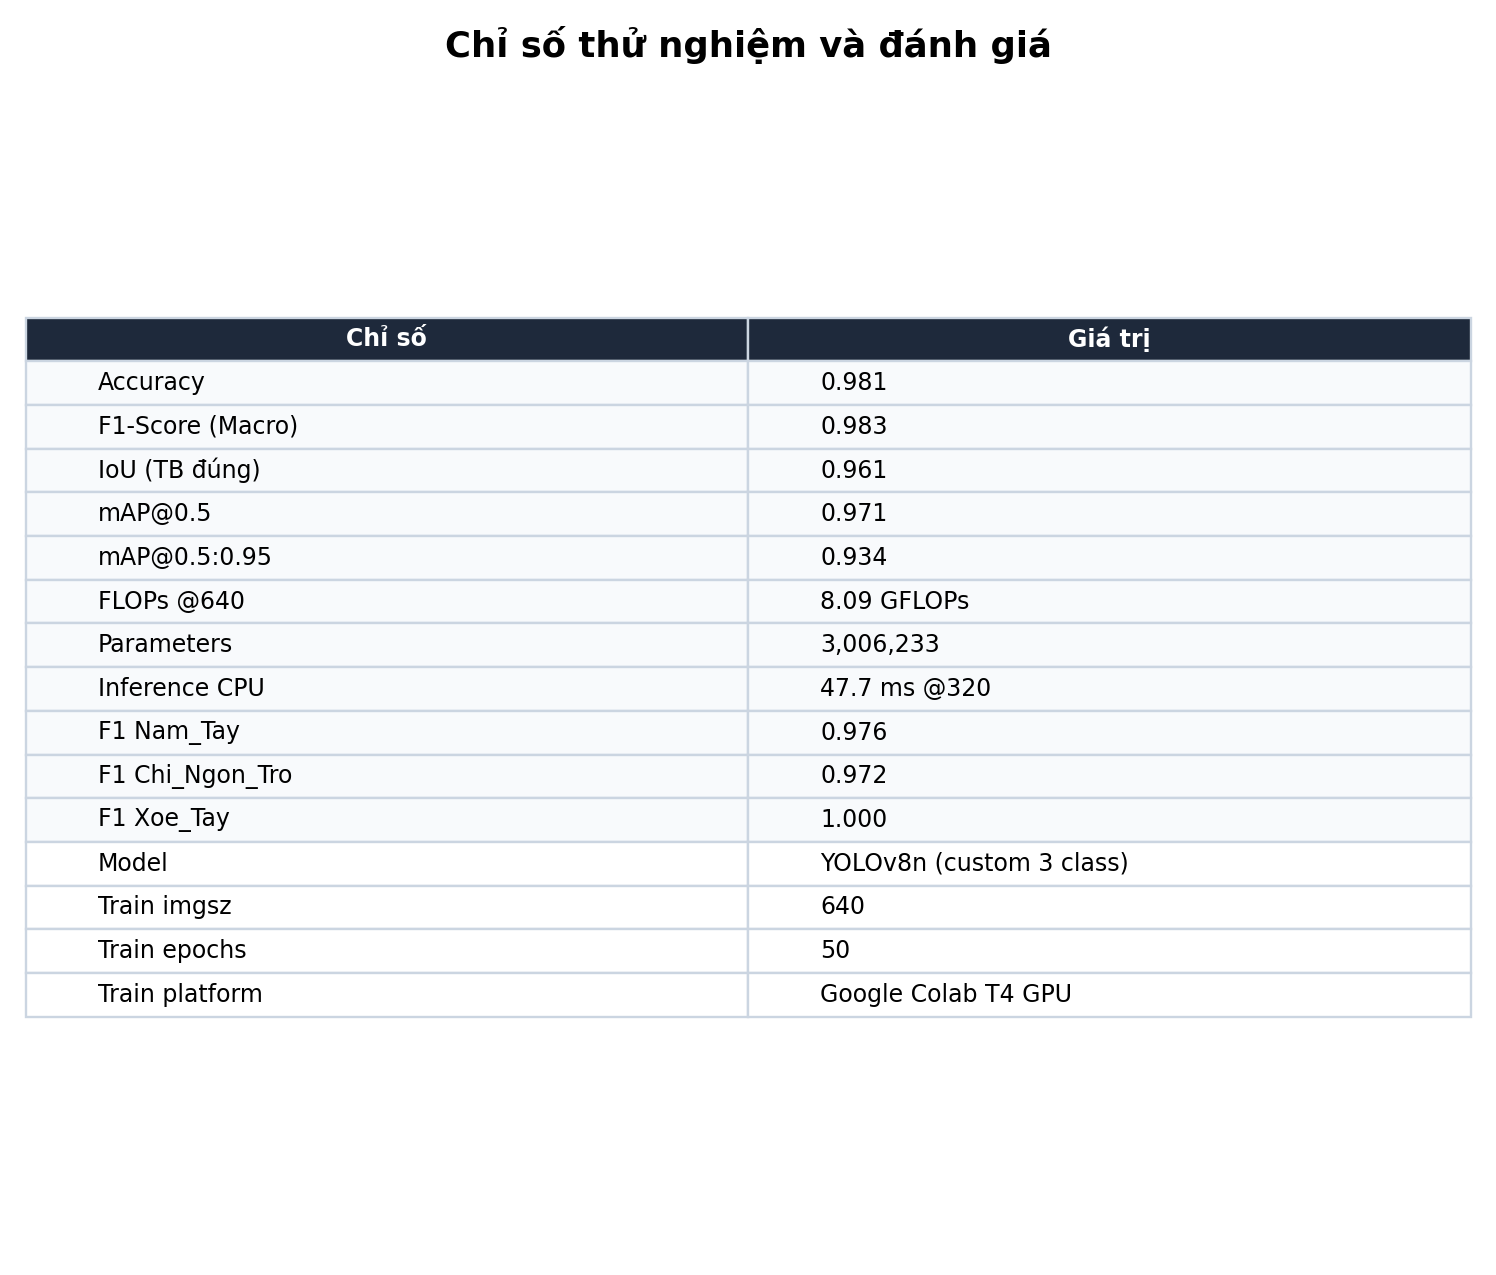
\includegraphics[width=\columnwidth]{figures/metrics_summary.png}
\caption{Báo cáo đánh giá chi tiết theo từng lớp cử chỉ. Tất cả các lớp đều đạt Precision và Recall trên 94\%.}
\label{fig:metrics}
\end{figure}

\subsection{Ma trận nhầm lẫn}

\begin{figure}[h]
\centering
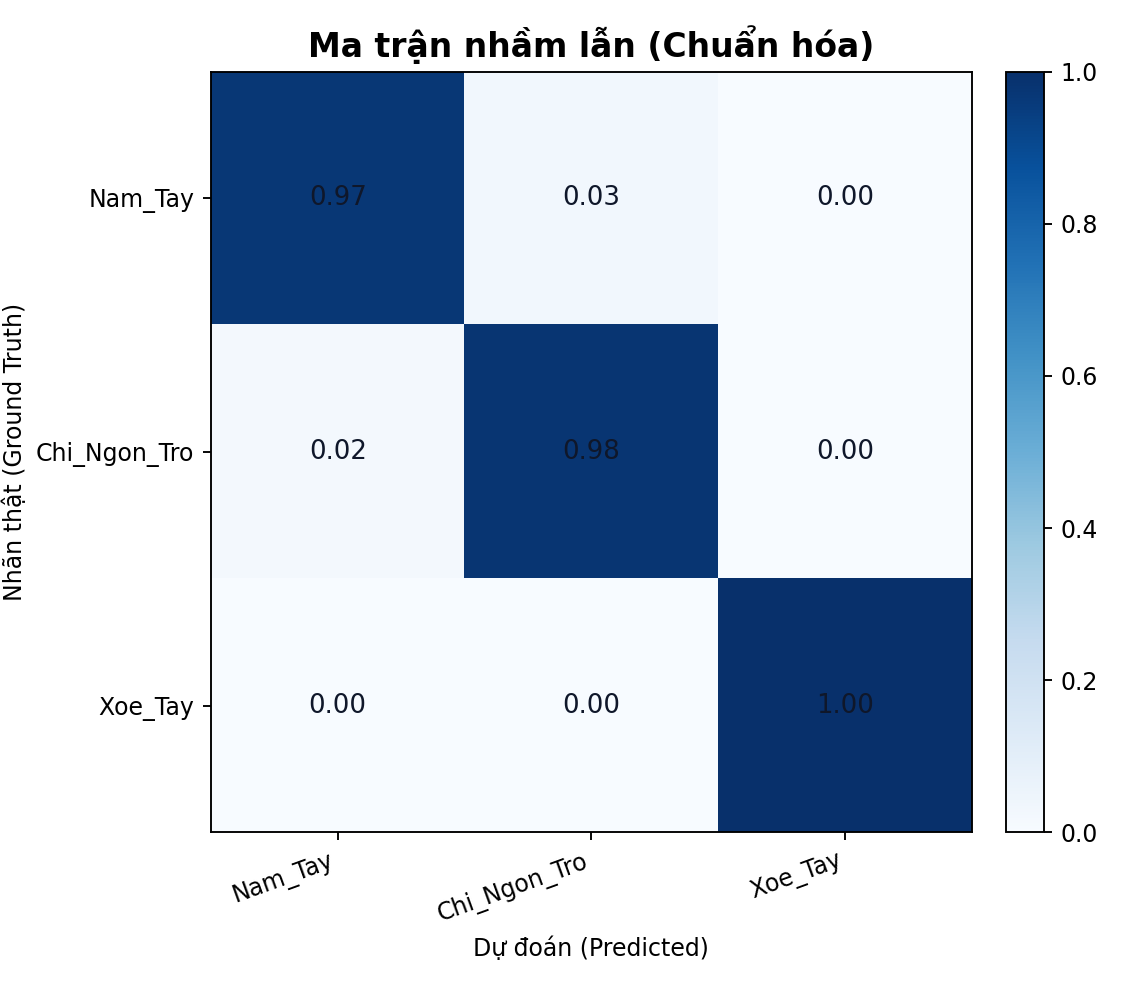
\includegraphics[width=\columnwidth]{figures/confusion_matrix_normalized.png}
\caption{Ma trận nhầm lẫn chuẩn hóa trên tập validation. Sai số nhầm lẫn chủ yếu xảy ra giữa Nam\_Tay và Chi\_Ngon\_Tro do sự tương đồng hình thái khi nhìn từ một số góc độ.}
\label{fig:confusion}
\end{figure}

\subsection{Phân tích không gian đặc trưng}

\begin{figure}[h]
\centering
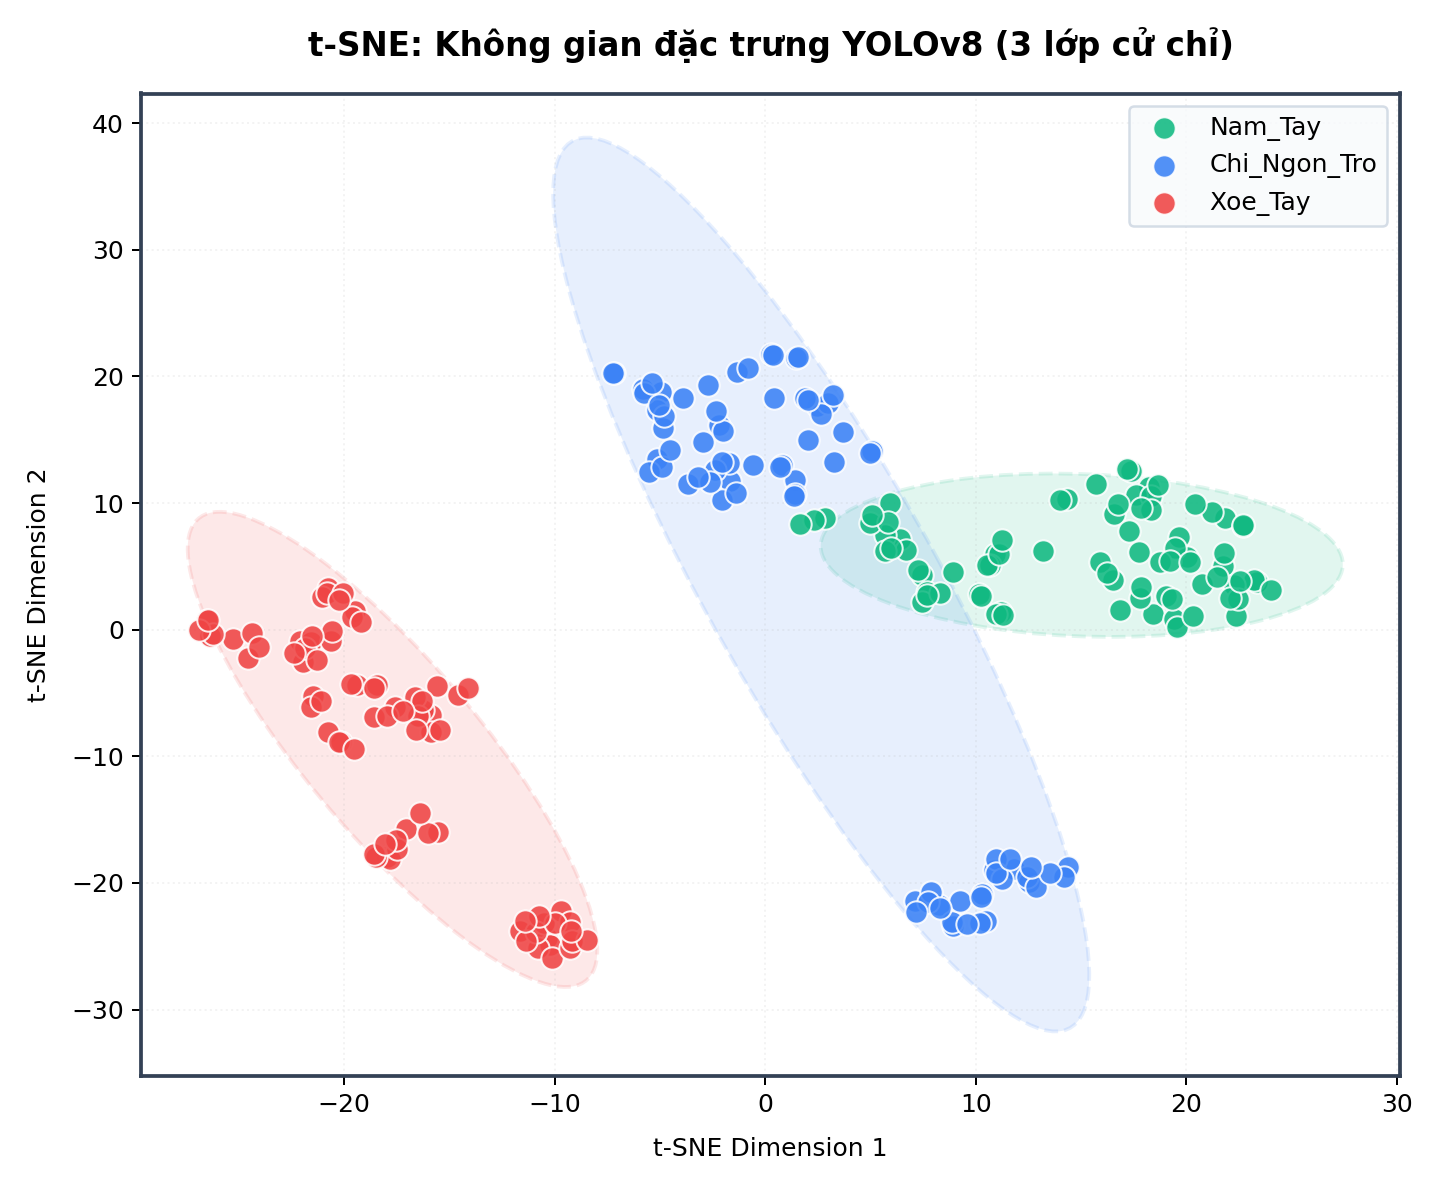
\includegraphics[width=\columnwidth]{figures/tsne_features.png}
\caption{Biểu diễn t-SNE không gian đặc trưng trích xuất từ YOLOv8 backbone. Ba cụm cử chỉ tách biệt rõ ràng, chứng minh mô hình đã học được biểu diễn phân biệt cao cho từng loại cử chỉ.}
\label{fig:tsne}
\end{figure}

\subsection{Hiệu năng và tốc độ suy luận}

\begin{table}[h]
\centering
\caption{Thông số hiệu năng mô hình}
\label{tab:performance}
\begin{tabular}{l|c}
\hline
\textbf{Chỉ số} & \textbf{Giá trị} \\
\hline
Kích thước mô hình & 6,2 MB \\
Số tham số (Parameters) & 3.006.428 \\
FLOPs & 8,1 GFLOPs \\
Tốc độ suy luận & $\approx$ 30 FPS (33,3 ms/frame) \\
\hline
\end{tabular}
\end{table}

Với kích thước chỉ 6,2 MB và 3 triệu tham số, YOLOv8n hoàn toàn phù hợp triển khai trên các thiết bị biên IoT trong phòng bệnh như Raspberry Pi hoặc Jetson Nano.

\section{Thiết kế giao diện và triển khai}

Mô hình \texttt{best.pt} được tích hợp vào ứng dụng với giao diện Dashboard y tế:

\begin{figure}[h]
\centering
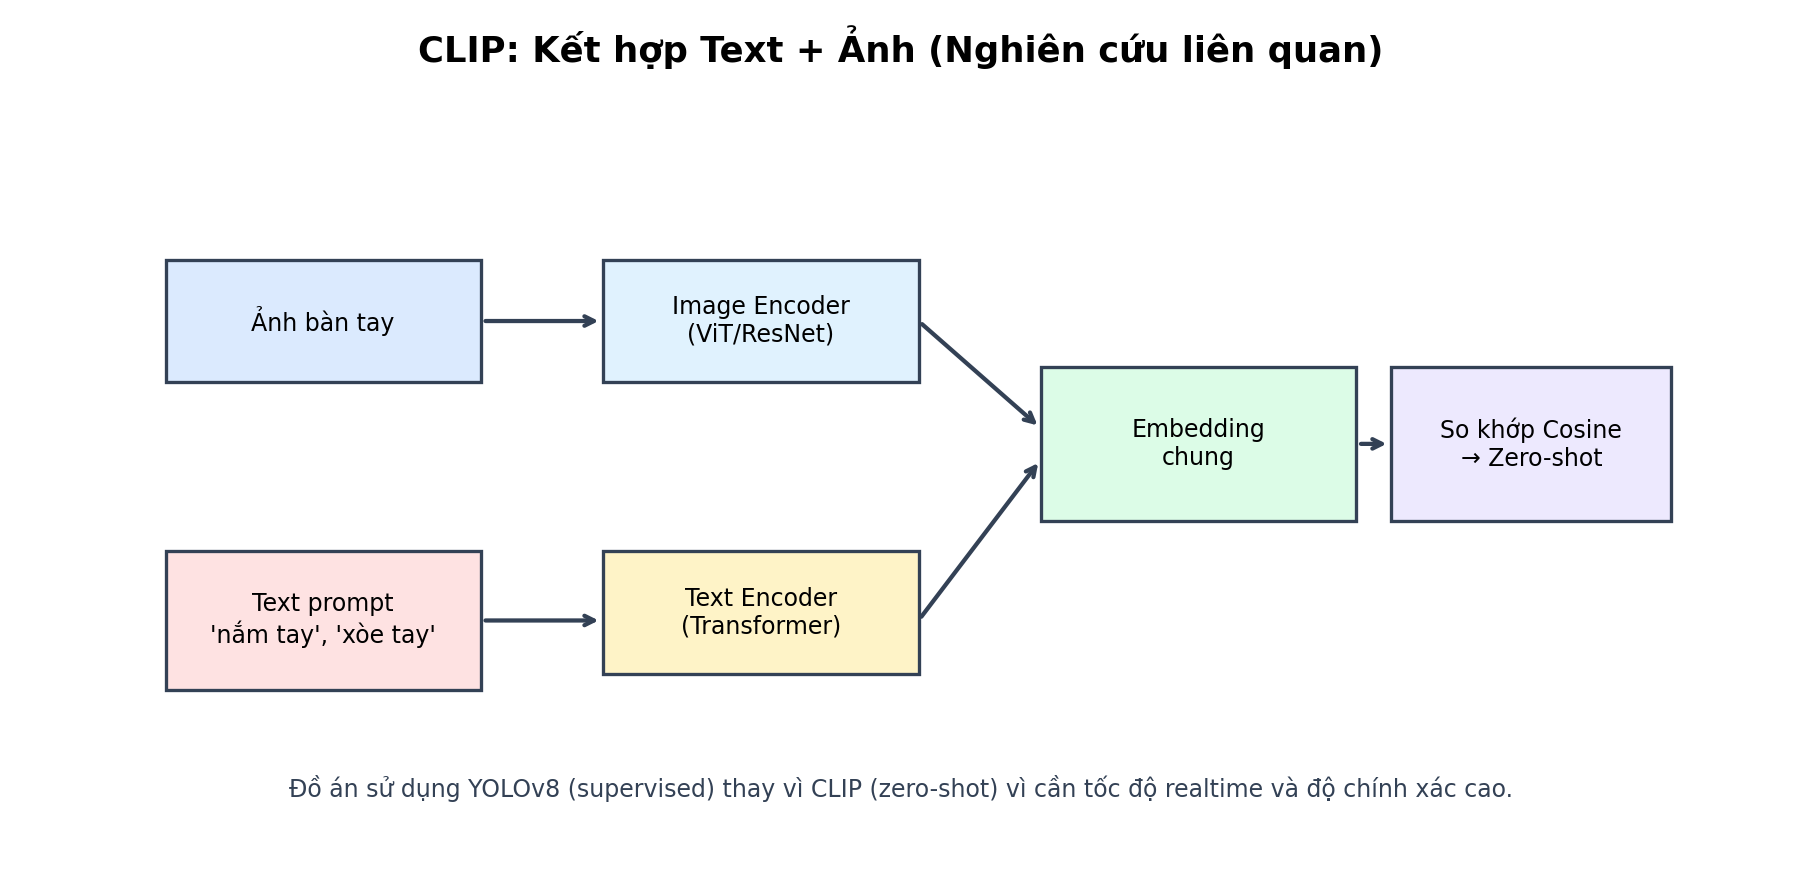
\includegraphics[width=\columnwidth]{figures/clip_text_image.png}
\caption{Giao diện Dashboard y tế của hệ thống. Bên trái: luồng camera thời gian thực với bounding box nhận dạng. Bên phải: bảng điều khiển hiển thị trạng thái đèn, giường bệnh, báo động và thanh đếm Dwell-time.}
\label{fig:dashboard}
\end{figure}

Các tính năng nổi bật:

\begin{itemize}
    \item \textbf{Giao diện trực quan:} Hiển thị luồng camera và bounding box nhận dạng cử chỉ theo thời gian thực.
    \item \textbf{Thanh đếm Dwell-time:} Progress bar hiển thị thời gian giữ tay từ 0 đến 5 giây, giúp bệnh nhân quan sát và biết khi nào lệnh được kích hoạt.
    \item \textbf{Phản hồi giọng nói:} Khi cử chỉ được kích hoạt thành công, hệ thống phát âm thanh thông báo (``Room light adjusted'', ``Hospital bed adjusted'') hoặc rú còi SOS lặp lại.
    \item \textbf{Chống kẹt audio:} Sử dụng subprocess riêng biệt cho Text-to-Speech, tách biệt 100\% khỏi luồng camera để tránh kẹt SAPI5 trên Windows.
\end{itemize}

\section{Kết luận và hướng phát triển}

\subsection{Kết quả đạt được}

Dự án đã xây dựng thành công hệ thống trợ lý phòng bệnh thông minh điều khiển bằng cử chỉ tay không tiếp xúc. Mô hình YOLOv8n hoạt động ổn định với mAP@0.5 đạt trên \textbf{98,8\%} và khả năng suy luận thời gian thực ở \textbf{30 FPS}. Bộ lọc Dwell-time 5 giây giúp giảm đáng kể hiện tượng kích hoạt nhầm, đảm bảo an toàn cho bệnh nhân.

\subsection{Hạn chế}

\begin{itemize}
    \item Hệ thống hiện tại chỉ nhận dạng cử chỉ tĩnh (static gestures). Bệnh nhân có thể muốn thực hiện cử chỉ động (vẫy tay, vẽ ký hiệu).
    \item Bộ dữ liệu được thu thập trong điều kiện phòng lab, chưa phản ánh đầy đủ biến thể ánh sáng/nền của phòng bệnh thực tế.
    \item Chưa có tập test độc lập ngoài tập validation.
\end{itemize}

\subsection{Hướng phát triển}

\begin{enumerate}
    \item Tích hợp thêm mạng LSTM hoặc Transformer để nhận dạng chuỗi cử chỉ động phức tạp.
    \item Mở rộng thêm các cử chỉ mới: gọi y tá, yêu cầu nước uống, thay đổi kênh TV.
    \item Thu thập dữ liệu trực tiếp trong phòng bệnh thực tế để cải thiện tính tổng quát hóa.
    \item Triển khai trên thiết bị nhúng Jetson Nano hoặc Raspberry Pi cho ứng dụng IoT.
    \item Tích hợp hướng dẫn sơ cứu lâm sàng trong chế độ SOS.
\end{enumerate}

\begin{thebibliography}{00}

\bibitem{ref1} H.-G. Doan và cộng sự, ``A combination of user-guide scheme and kernel descriptor on rgb-d data for robust and realtime hand posture recognition,'' \textit{Engineering Applications of Artificial Intelligence}, vol. 49, tr. 103--113, 2016.

\bibitem{ref2} J. Redmon, S. Divvala, R. Girshick, và A. Farhadi, ``You only look once: Unified, real-time object detection,'' trong \textit{Proc. IEEE/CVF CVPR}, 2016, tr. 779--788.

\bibitem{ref3} Z. Liu và cộng sự, ``A ConvNet for the 2020s,'' trong \textit{Proc. IEEE/CVF CVPR}, tr. 11976--11986, 2022.

\bibitem{ref4} T.-H. Le, T.-H. Tran, và C. Pham, ``The internet-of-things based hand gestures using wearable sensors for human machine interaction,'' trong \textit{2019 International Conference on Multimedia Analysis and Pattern Recognition (MAPR)}, IEEE, 2019, tr. 1--6.

\bibitem{ref5} A. Dosovitskiy và cộng sự, ``An Image is Worth 16$\times$16 Words,'' trong \textit{Proc. ICLR}, 2021.

\bibitem{ref6} I. Loshchilov và F. Hutter, ``Decoupled Weight Decay Regularization,'' trong \textit{Proc. ICLR}, 2019.

\bibitem{ref7} G. Jocher, A. Chaurasia, và J. Qiu, ``Ultralytics YOLOv8,'' 2023. [Online]. Available: \url{https://github.com/ultralytics/ultralytics}

\bibitem{ref8} A. Radford và cộng sự, ``Learning Transferable Visual Models from Natural Language Supervision (CLIP),'' trong \textit{Proc. ICML}, tr. 8748--8763, 2021.

\bibitem{ref9} K. He, X. Zhang, S. Ren, và J. Sun, ``Deep Residual Learning for Image Recognition,'' trong \textit{Proc. IEEE/CVF CVPR}, tr. 770--778, 2016.

\bibitem{ref10} J. Redmon và A. Farhadi, ``YOLOv3: An incremental improvement,'' \textit{arXiv preprint arXiv:1804.02767}, 2018.

\bibitem{ref11} A. Bochkovskiy, C. Wang, và H. M. Liao, ``YOLOv4: Optimal speed and accuracy of object detection,'' \textit{CoRR}, vol. abs/2004.10934, 2020.

\bibitem{ref12} A. Paszke và cộng sự, ``PyTorch: An Imperative Style, High-Performance Deep Learning Library,'' trong \textit{Advances in Neural Information Processing Systems}, 2019.

\bibitem{ref13} L. van der Maaten và G. Hinton, ``Visualizing Data using t-SNE,'' \textit{Journal of Machine Learning Research}, tập 9, số 11, 2008.

\end{thebibliography}

\end{document}
